\chapter{Grundlagen}
\section{Ermüdigungstest}
Die meisten Bauteilkonstruktionen beinhalten Komponenten, die zyklischen Belastungen ausgesetzt sind. Zyklische Belastungen führen zu Schwankungen oder zyklischen Spannungen, die häufig zu Ermüdungsversagen führen können. Mit der starken Entwicklung der Eisenbahn in der Mitte des 19. Jahrhunderts wurde das Ermüdungsversagen bei Eisenbahnachsen zu einem weit verbreiteten Problem. Daher wurde die Notwendigkeit, das Versagensverhalten von Materialien unter wiederholten Belastungen zu verstehen, besonders deutlich. Zwischen 1852 und 1870 führte August Wöhler die ersten dokumentierten Ermüdungsversuche an Eisenbahnachsen durch, die Millionen von Lastzyklen bei Spannungspegeln erlebten, die weit unterhalb der monotonen Zugfestigkeit lagen \cite{august_wöhler}. Heutzutage werden Ermüdungstests in verschiedenen Branchen wie Materialwissenschaft, Ingenieurwissenschaft, Luft- und Raumfahrt sowie Fahrzeugbau eingesetzt, um die Lebensdauer und Zuverlässigkeit von Produkten zu bestimmen. Typischerweise werden diese Tests durchgeführt, indem man das Material oder die Struktur wiederholt Belastungen aussetzt, die denen ähneln, die im realen Betrieb auftreten können. Dies ermöglicht es, potenzielle Schwachstellen oder Versagensmechanismen vom Material zu identifizieren und entsprechende Maßnahmen zur Verbesserung der Haltbarkeit zu ergreifen. 

Ermüdungstests werden in der Regel mithilfe von dynamischer Zugprüfmaschinen durchgeführt, die in der Lage sind, große, amplitudenzyklische Lasten aufzubringen. Die Ermüdungslebensdauer einer Probe ist die Anzahl der Zyklen, die es dauert, bis die Probe versagt. Diese Daten können zur Erstellung von Wöhler-, S-N-, oder Spannungs-Lebensdauer-Kurven \ref{fig:background:Lebensdauer-Kurven} verwendet werden \cite{fatigue_test}. Wie in Abbildung \ref{fig:background:Lebensdauer-Kurven} zu sehen ist, gibt es drei Bereiche. Im Bereich der Kurzfestigkeit werden die Proben so stark belastet, dass sie bereits nach wenigen Zyklen versagen. Wenn die Proben weniger beansprucht werden, benötigen sie mehr Zyklen, um zu versagen, und befinden sich daher im Bereich der Zeitfestigkeit. Bei Beanspruchungen in diesem Bereich kann ein Bauteil betriebsfest ausgelegt werden. Im Bereich der Dauerfestigkeit treten fast keine Risse mehr auf, und die Wöhlerkurve nähert sich horizontal an. Die Form der Wöhlerkurve variiert abhängig vom Material und kann als Vergleichsmaßstab von Versagensmechanismen zwischen verschiedenen Materialien dienen. 

\begin{figure}[htbp]
 \centering
 \includegraphics[width=0.7\textwidth]{gfx/FatigueTest/WöhlerCurve.png}
 \caption[Wöhlerkurve in Ermüdungstests]{Das Ergebnis eines Ermüdungstests wird in Wöhlerkurve Diagramm mit y Achse als die zyklische Spannungsamplitude und x Achse als die Anzahl der Zyklen bis zum Versagen dargestellt. Die Datenpunkte nennt man Ermüdungspunkte, an denen eine Probe versagt. Die Wöhlerkurve wird durch eine Regression durch diese Punkte erzeugt. Quelle: Eigene Quelle}
 \label{fig:background:Lebensdauer-Kurven}
\end{figure}

Eine dynamische Zugprüfmaschiene \ref{fig:background:DynamischeZugprüfmaschiene} besteht allgemein aus einem Rahmen, der mit einer Kraftmesszelle, einer statischen Traverse (Spannvorrichtung oder Probenhalter) und einer dynamischen Traverser ausgestattet ist. Während des Tests  bewegt sich die dynamische Traverse mit der eingestellten Geschwindigkeit, was dazu führt, dass die Probe einer Zugkraft ausgesetzt wird, um ihre Belastungsgrenzen zu erreichen und letztendlich zu brechen. Die gleichzeitig auftretende Verformung der Probe - entweder durch Messung entlang des Traversenwegs oder mithilfe eines Dehnungssensors - und die darauf wirkende Kraft werden durch Kraftmesszelle kontinuierlich gemessen und aufgezeichnet. Eine typische Testprobe hat eine runde Sanduhr-Form für Metall und eine flache Sanduhr-Form für Gummi.

\begin{figure}[htbp]
    \centering
        \subfigure[]{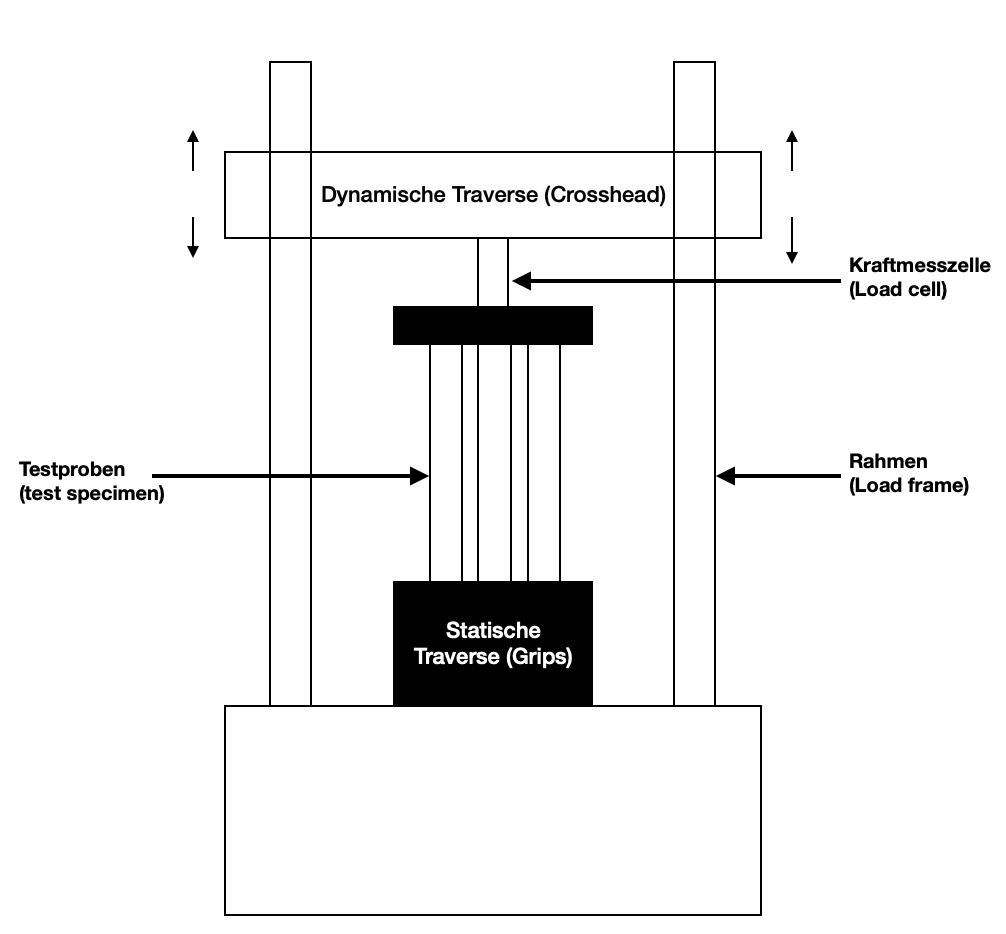
\includegraphics[width=0.49\textwidth, height=0.45\textwidth]{gfx/FatigueTest/TestMaschine.png}}
        \subfigure[]{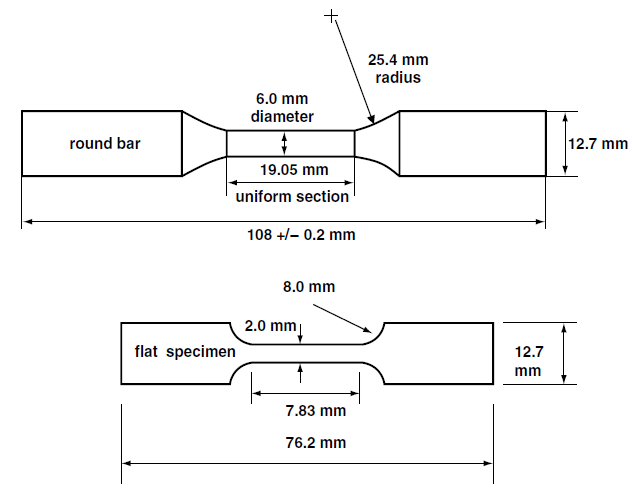
\includegraphics[width=0.49\textwidth, height=0.45\textwidth]{gfx/FatigueTest/Specimens.png}}
 \caption[Dynamische Zugprüfmaschiene und Testproben]{(a) Dynamische Zugprüfmaschine mit vier Hauptkomponenten: Die Testproben werden zwischen zwei Traversen gedehnt und gedrückt, bis sie reißen. Dabei misst eine Kraftmesszelle die auf das Crosshead ausgeübte Kraft. Quelle: Eigene Quelle. (b) Ein Beispiel für die typische Form von Testproben. Quelle: \cite{specimens}.}
 \label{fig:background:DynamischeZugprüfmaschiene}
\end{figure}

\section{Neural Network}
Ein neuronales Netzwerk ist ein Rechenmodell, das durch die Struktur und Funktionsweise des menschlichen Gehirns inspiriert wurde. Diese innovative Idee wurde erstmals im Jahr 1943 von Warren McCulloch, einem Neurophysiologen, und Walter Pitts, einem Mathematiker, präsentiert \cite{McCullock1943}. In ihrer Arbeit entwickelten sie vernetzte Schaltkreise, um die grundlegenden Konzepte der Nervensystemaktivität zu erfassen, und legten somit den Grundstein für künstliche neuronale Netzwerke. Erst in den letzten Jahrzehnten gewannen neuronale Netzwerke aufgrund signifikanter Fortschritte in Rechenleistung und einer enormen Zunahme an verfügbaren Trainingdaten (wie ImageNet \cite{imagenet}) zunehmend an Bekanntheit. Heutzutage sind neuronale Netzwerke dominierend im Bereich des Visual Computing, Natural Language Processing und vielen anderen Anwendungen.

    \subsection{Perceptron}
    In den 1950er und 1960er Jahren präsentierte der Psychologe Frank Rosenblatt das Konzept des Perceptrons, das auf dem McCulloch-Pitts-Neuron basiert und als Grundbaustein für spätere, komplexere Netzwerke dient \cite{rosenblatt}. Ein Perceptron \ref{tab:background:Perceptron} nimmt dabei mehrere Eingaben (x1, x2, ...) mit entsprechenden Gewichten (w1, w2, ...) entgegen und gibt einen Ausgabe Y aus . Die Verbindungen zwischen den Perceptronen variieren je nach Netzstruktur. Nach Rosenblatt ist der Ausgabe ''0'' oder ''1'' (ausgelöst), abhängig davon, ob die gewichtete Summe der Eingaben kleiner oder größer als ein Theshold ist. Anders ausgedrückt haben die Verbindungen zwischen den Perceptronen unterschiedliche Gewichte und beeinflussen somit den Ausgang eines jeden Perceptrons. Dieses Konzept von Rosenblatt spiegelt den Mechanismus des menschlichen Gehirns wider, in dem sich neuronale Verbindungen bei jeder aufeinanderfolgenden Verwendung verstärken, insbesondere zwischen Neuronen, die dazu neigen, gleichzeitig aktiv zu werden \cite{organization-of-behavior-1949}.

    \begin{table}[htbp]
        \begin{tabular}{c c}
            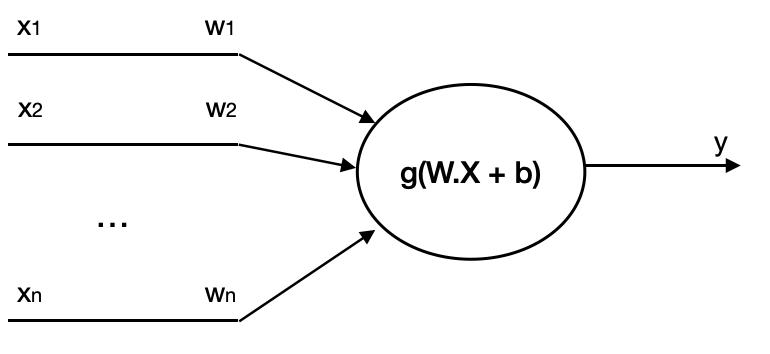
\includegraphics[width=0.5\linewidth, height=0.25\textwidth, valign=m]{gfx/NeuralNet/Perceptron.png}
            &
            $y = \begin{cases}
                0 & \text{if } W.X - threshold \le 0. \\
                1 & \text{otherwise}.
                 \end{cases}
            $  
        \end{tabular}
        \caption[Perceptron]{\textbf{Links}: Ein Perceptron generiert eine Ausgabe y, die durch die Aktivierungsfunktion $g(x)$ berechnet wird. Die Aktivierungsfunktion $g(x)$ erhält das Skalarprodukt des Eingangsvektors $X$ und des Gewichtsvektors $W$, zuzüglich eines Bias $b$ des entsprechenden Perceptrons als Eingabe. Das Bias $(b = - threshold)$ gibt im einfachen Wort an, wie leicht das entsprechende Perceptron ausgelöst wird, also eine ''1'' ausgibt. \textbf{Rechts}: die Aktivierungsfunktion nach Rosenblatt.}
        \label{tab:background:Perceptron}
    \end{table}

   Die Aktivierungsfunktion eines Perceptrons definiert, wie es aktiviert wird und welchen Ausgabewert es erzeugt. Es gibt mehrere Aktivierungsfunktionen, von denen jede ihre eigenen Vor- und Nachteile hat und je nach Anwendung ausgewählt werden kann. Die Threshold-Version der Aktivierungsfunktion (auch als Treppenfunktion bekannt) von Rosenblatt hat einen signifikanten Nachteil: Die Ausgabewerte können nur 0 oder 1 sein, was zu Diskontinuität und mangelnder Differenzierbarkeit führt. Dies begrenzt die Fähigkeit von Perceptrons, nichtlinear separierbare Klassen zu erkennen, was in komplexeren realen Problemen oft der Fall ist. Um diese Einschränkung zu überwinden, wurden später nichtlineare Aktivierungsfunktionen eingeführt, darunter die Sigmoid-Funktion, die hyperbolische Tangensfunktion (tanh), die Rektifizierte Lineare Einheitsfunktion (Rectified Linear Unit - ReLU) usw.  \ref{fig:background:Aktivierungsfunktionen}.   

    \begin{figure}[htbp]
    \centering
        \subfigure{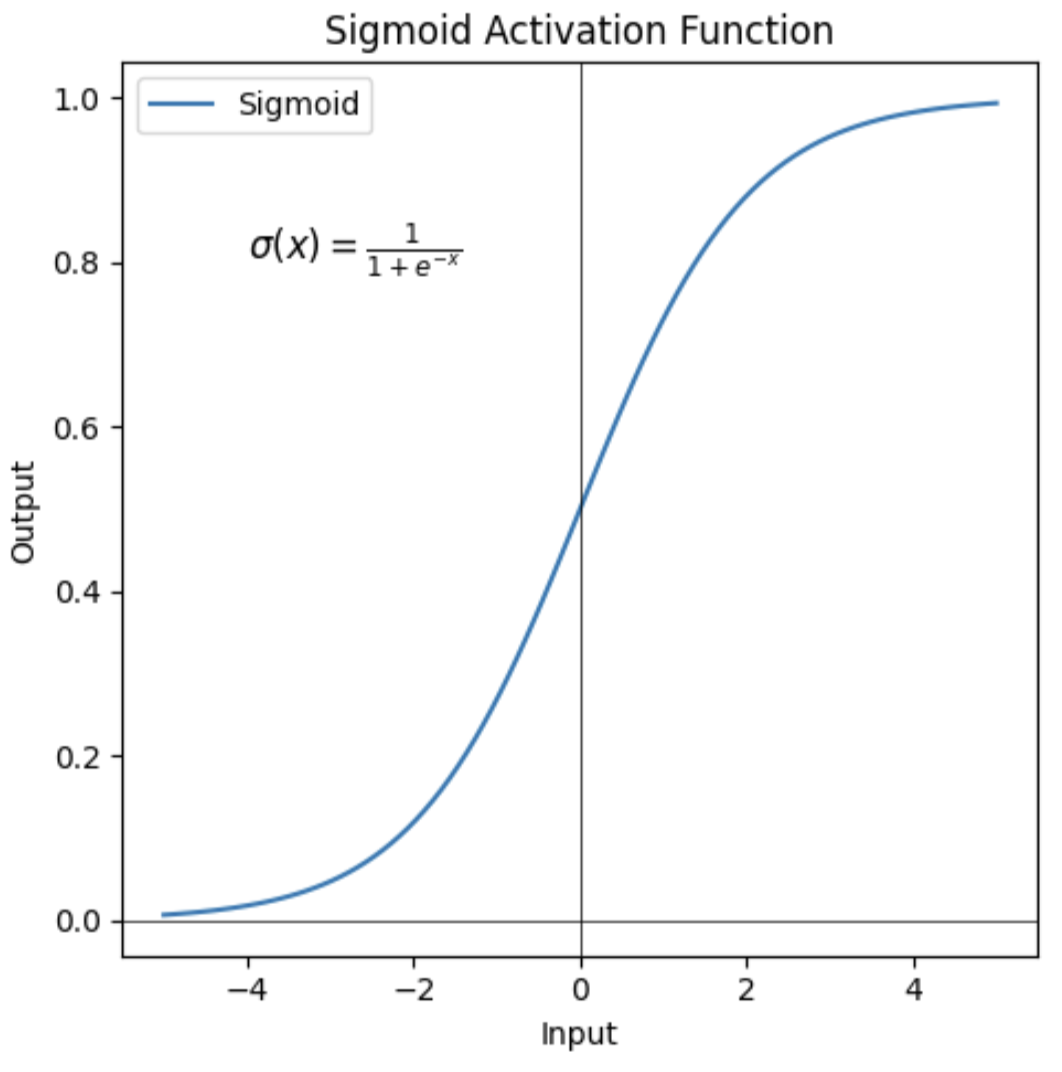
\includegraphics[width=0.32\linewidth, height=0.33\linewidth]{gfx/NeuralNet/Sigmoid.png}}
        \subfigure{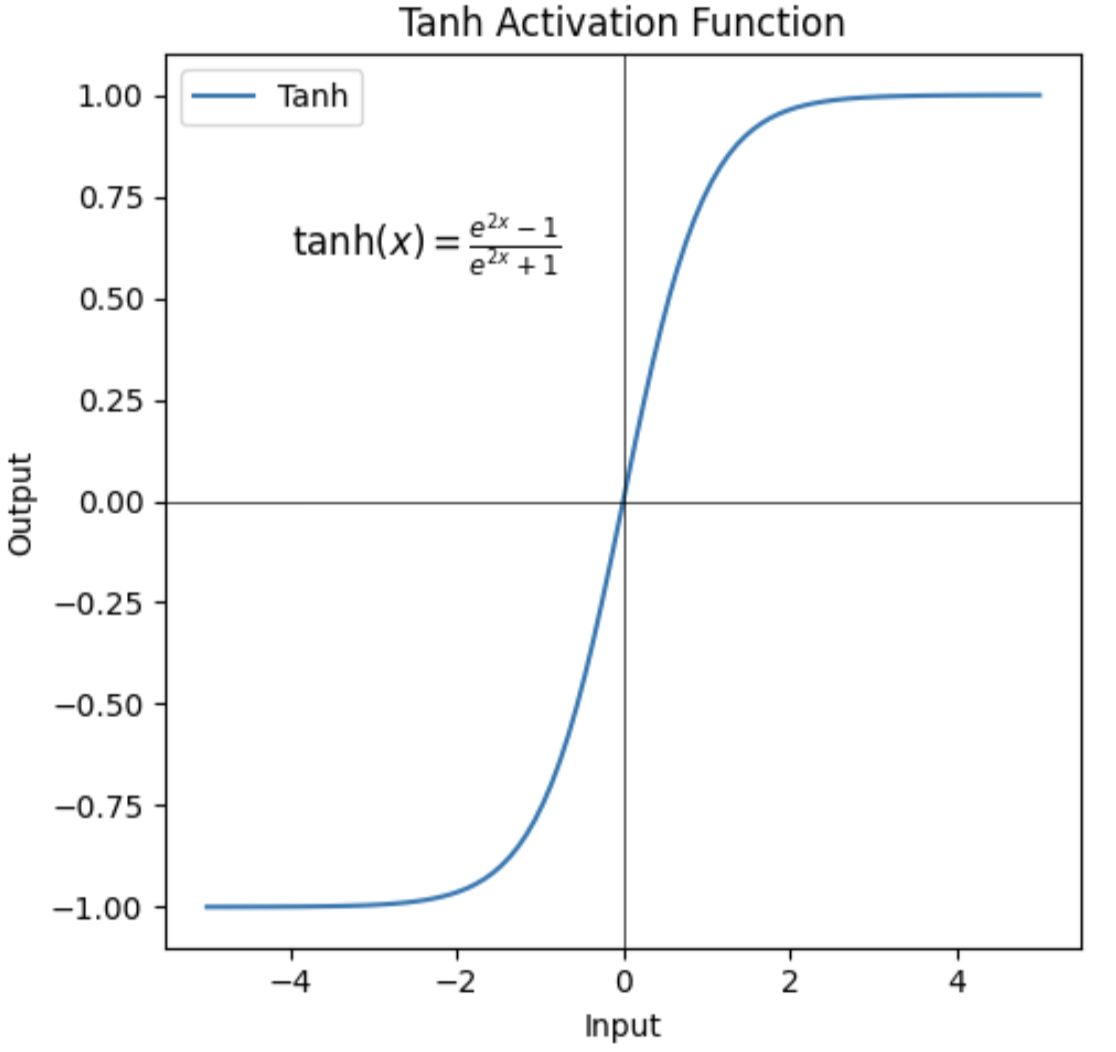
\includegraphics[width=0.32\linewidth, height=0.33\linewidth]{gfx/NeuralNet/Tanh.png}}
        \subfigure{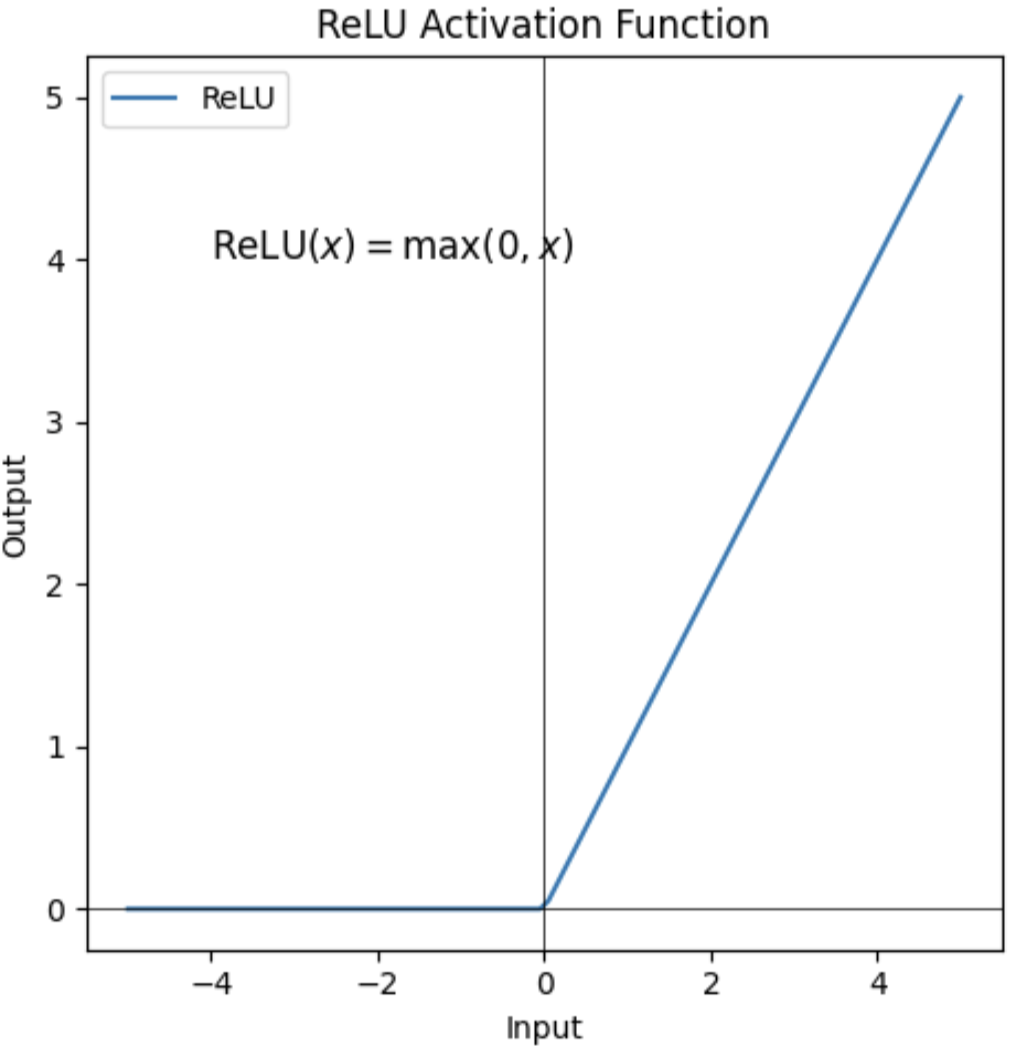
\includegraphics[width=0.32\linewidth, height=0.33\linewidth]{gfx/NeuralNet/ReLU.png}}
        \caption[Aktivierungsfunktionen]{Hier sind drei Beispiele für häufig verwendete Aktivierungsfunktionen in modernen neuronalen Netzwerken. Alle drei Funktionen sind sowohl differenzierbar als auch kontinuierlich.}
        \label{fig:background:Aktivierungsfunktionen}
    \end{figure}

    Die Sigmoid-Funktion erzeugt Ausgabewerte im Bereich von 0 bis 1, was sie besonders gut für die Vorhersage von Wahrscheinlichkeiten macht. Häufig wird sie in Klassifizierungsaufgaben eingesetzt, wo das Ergebnis angibt, wie wahrscheinlich es ist, dass die Eingabe zu einer bestimmten Klasse gehört (1 für 100 \% Übereinstimmung und 0 für gar keine Übereinstimmung). Die Tanh-Funktion ist eine Erweiterung der Sigmoid-Funktion, da sie auch negative Ausgabewerte erzeugt. Die ReLU-Funktion wird weitgehend im Bereich des Deep Learnings, insbesondere in Convolutional Neural Networks (CNNs), verwendet. Ihr Vorteil liegt in ihrer Einfachheit (sie gibt entweder 0 oder $ x $ zurück, abhängig vom Vorzeichen der Eingabe), wodurch sie schnell berechnet werden kann. In tiefen neuronalen Netzwerken, in denen Modelle oft groß und komplex sind und mit großen Datenmengen trainiert werden, spielt die Rechenleistung eine entscheidende Rolle. 

    \subsection{Architektur}
    Ein neuronales Netzwerk besteht aus drei Haupttypen von Schichten: dem Eingangsschict (Input Layer), den versteckten Schichten (Hidden Layer) und dem Ausgangsschicht (Output Layer). Es gibt zwei grundlegende Typen von neuronalen Netzwerken: Single-Layer neuronale Netzwerke und Multilayer neuronale Netzwerke.

    Ein Single-Layer neuronale Netzwerk, wie in \ref{fig:background:SingleLayerNeuralNetwork} dargestellt, setzt sich aus einer Eingangsschicht, einer versteckten Schicht und einer Ausgangsschicht zusammen. Es empfängt einen Eingabevektor $I$ mit den Variablen $X_1, X_2, X_3, X_4$  in der Eingangsschicht. Der Ausgang $Y$ wird durch die Funktion $f(X)$ berechnet. Der Vektor $W$ enthält die Gewichte (auch als Parameter bezeichnet) zwischen der Eingangsschicht und der versteckten Schicht, während der Vektor $\beta$ die Gewichte zwischen der versteckten Schicht und der Ausgangsschicht repräsentiert. Das neuronale Netzwerk kann durch die Gleichung \ref{eq:background:SingleLayer} dargestellt werden \cite{introAI}. Dabei sind $\beta_0$ und $w_{k0}$ Bias des entsprechenden Perceptrons, und $g(x)$ repräsentiert die Aktivierungsfunktion dieses Perceptrons.
    
    \begin{equation}
        f(X) = \beta_0 + \sum_{k=1}^{K} \beta_k g(w_{k0} + \sum_{i=1}^{I} w_{ki} X_i)
    \label{eq:background:SingleLayer}
    \end{equation}

    \begin{figure}
        \centering
        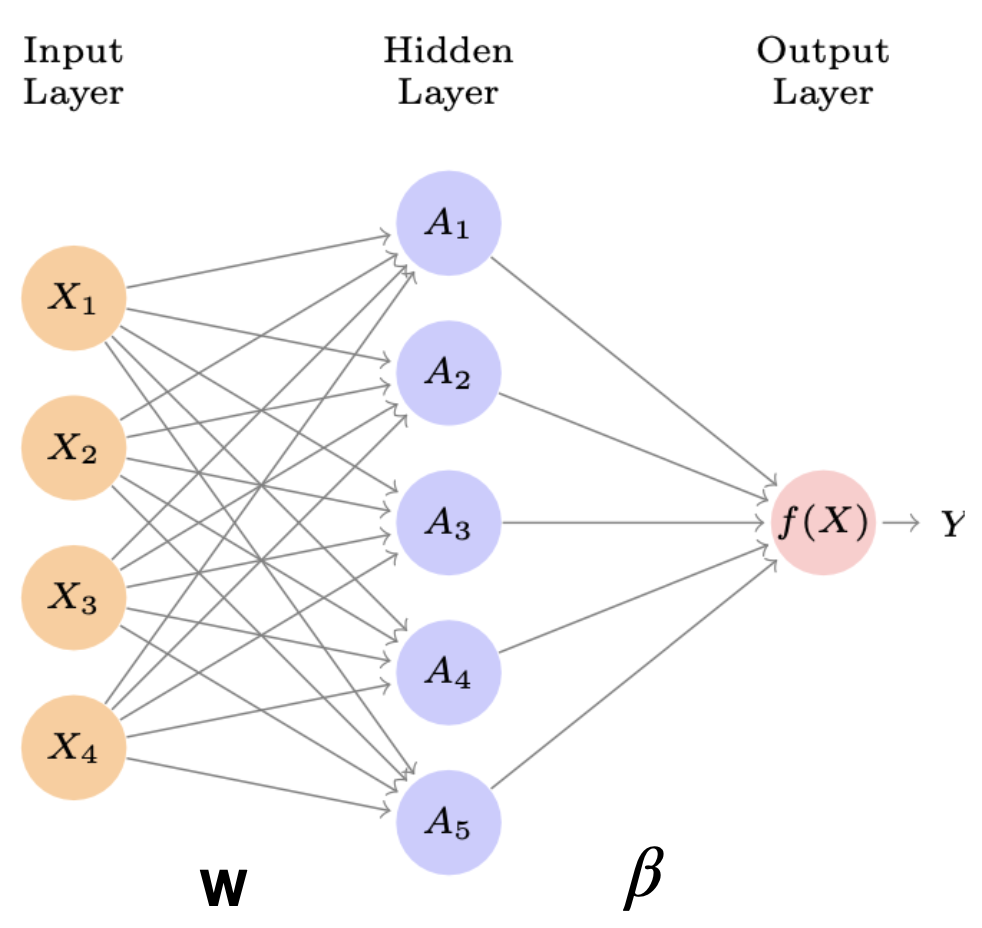
\includegraphics[width=0.5\linewidth]{gfx/NeuralNet/SingleLayer.png}
        \caption[Single-Layer neuronales Netzwerk]{Ein Single-Layer neuronales Netzwerk mit $I = 4$ Eingängen, einem Ausgang $Y = f(X)$, einer versteckten Schicht mit $K = 5$ Einheiten sowie zwei Gewichtsvektoren $W$ und $\beta$. Quelle: \cite{introAI}}
        \label{fig:background:SingleLayerNeuralNetwork}
    \end{figure}

    Ein Multilayer neuronales Netzwerk besteht aus einer Eingangsschicht, einer Ausgangsschicht und mehreren versteckten Schichten. Die Abbildung \ref{fig:background:MultilayerNeuronalesNetwerk} zeigt ein Beispiel für ein Multilayer neuronales Netzwerk, das für das MNIST-Problem (einen handgeschriebenen Datensatz) \cite{MNIST} verwendet wird. Das Modell hat eine Eingangsschicht mit $I = 784$ Einheiten, die der Anzahl der Pixel $28 x 28 = 784$ in jedem Eingangsbild des MNIST-Datensatzes entspricht. Es gibt zwei versteckte Schichten mit $K_1 = 256$ und $K_2 = 128$ Einheiten. Die Ausgangsschicht besteht aus 10 Einheiten, die den Zahlen von 0 bis 9 entsprechen.
    
    Die Werte der Einheiten in der ersten (Gleichung \ref{eq:background:Layer1}) und zweiten (Gleichung \ref{eq:background:Layer2}) versteckten Schicht werden wie folgt berechnet \cite{introAI}:

    \begin{equation}
        A_{k_1}^{(1)} = g(w_{k_10}^{(1)} + \sum_{i = 1}^{I} w_{k_1i}^{(1)} X_i) 
    \label{eq:background:Layer1}
    \end{equation}

    \begin{equation}
        A_{k_2}^{(2)} = g(w_{k_20}^{(2)} + \sum_{j = 1}^{K_1} w_{k_2j}^{(2)} A_j^{(1)}) 
    \label{eq:background:Layer2}
    \end{equation}

    Jede Einheit $m \in {0, 1, ..., 9}$ in der Ausgangsschicht wird als das Ergebnis der Funktion $f_m(X)$ berechnet \cite{introAI}. Hierbei kann die Sigmoid-Funktion in der zweiten versteckten Schicht $A^{(2)}$ verwendet werden, um die Wahrscheinlichkeit zu berechnen, dass die Eingabe zu der entsprechenden Zahl gehört.

    \begin{equation}
        f_m(X) = \beta_{m0} + \sum_{k = 1}^{K_2} \beta_{mk} A_j^{(2)} 
    \label{eq:background:Layer2}
    \end{equation}

    \begin{figure}[htbp]
        \centering
        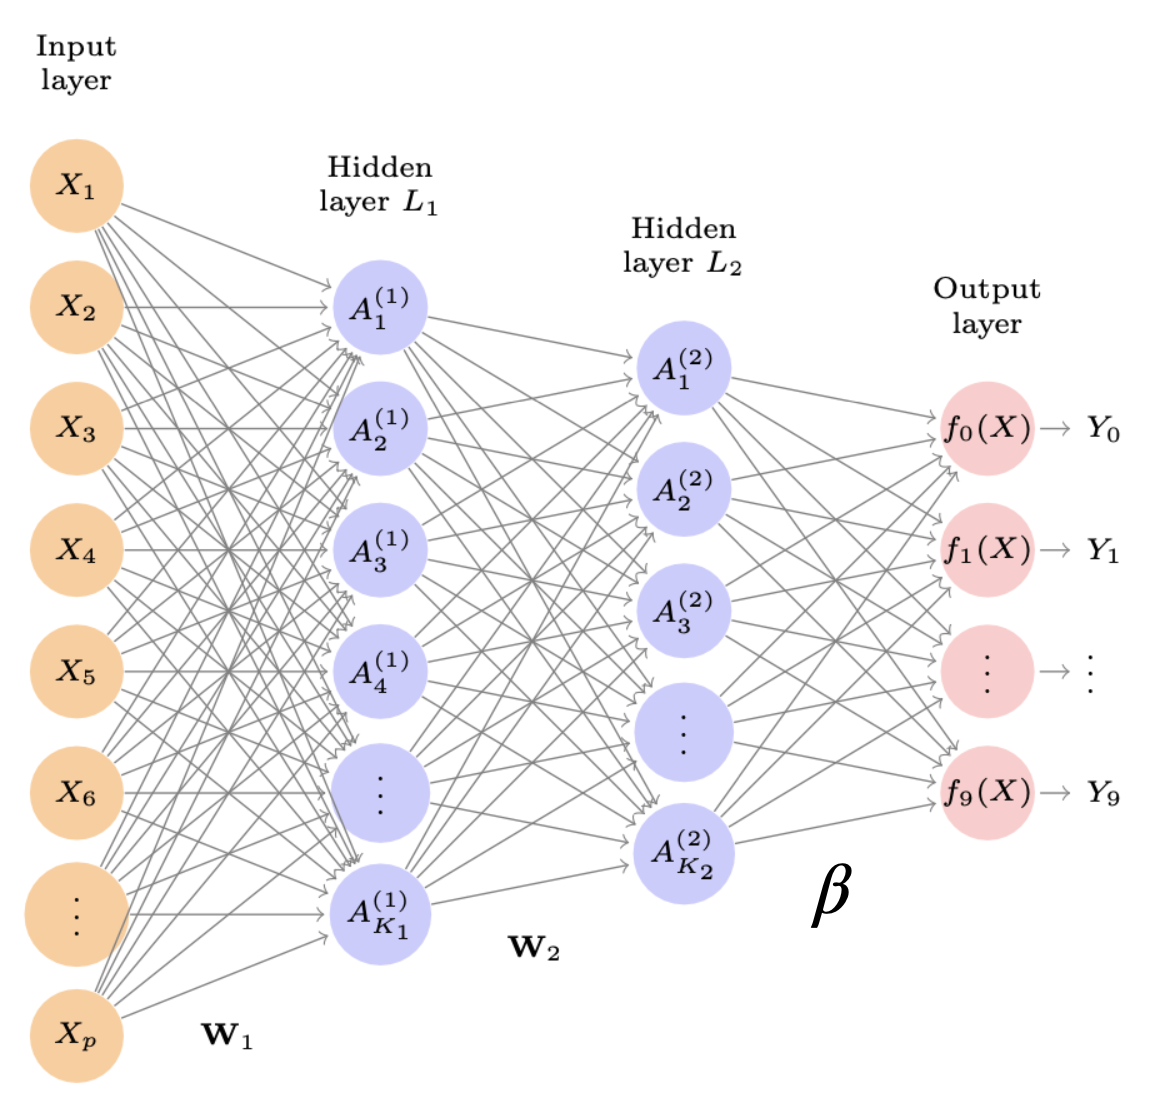
\includegraphics[width=0.6\linewidth]{gfx/NeuralNet/MultiLayer.png}
        \caption[Multilayer neuronales Netzwerk]{Ein Multilayer neuronales Netzwerk mit 2 versteckten Schichten für MNIST Problem mit $I = 784$ Einheiten in der Eingangsschicht, $K_1 = 256$ und $K_2 = 128$ Einheiten in zwei versteckten Schichten und $m = 10$ Einheiten in Ausgangsschicht. Insgesamt verfügt das Modell über 235.146 trainierbare Parameter, einschließlich Gewichte und Biases ($784 x 256 + 256 x 128 + 128 x 10 + 256 + 128 + 10 = 235146$). Quelle: \cite{introAI}}
        \label{fig:background:MultilayerNeuronalesNetwerk}
    \end{figure}

    \subsection{Gradient Descent}
\section{Convolutional Neural Network (CNN)}

\section{YOLO}
    \subsection{Intersection over Union}
    Die "Intersection over Union" (\acs{IoU}) oder der "Jaccard Index" ist eine Metrik, die in der Objekterkennung verwendet wird, um die Überlappung zwischen zwei Bounding-Boxen zu quantifizieren. Die \acs{IoU} wird durch die Division der Fläche der Überlappung zweier Bounding-Boxen durch die Fläche der Vereinigung dieser Bounding-Boxen berechnet. 

    \begin{equation}
        IoU(A, B) = \frac{|A \cap B|}{|A \cup B|}
    \end{equation}

    Hierbei repräsentiert A und B zwei Bounding-Boxes, $|x|$ die Fläche einer Bounding-Box, $\cap$ die Überlappung (Intersection) und $\cup$ die Vereinigung (Union).
\section{Kalman Filter}

\section{Bot-SORT}